\chapter{Temporal Property Detection with Numerical Dependencies and
Resampling}\label{chap:tempresult}

We now present results of our temporal logic for knowledge discovery
from NDs in temporal sequences applied to
real world data. In Section~\ref{sec:tr_intro} we discuss  the context
of our experiments and present the model for the discovery of
properties in Section~\ref{sec:tr_propmodel}. The model we provide,
given the flexibility of our logic, is not rigid and numerous
algorithms may be created to extend or diverge from this model. 
We present one algorithm in this context, noting that other algorithms
are direct implementations of the semantics provided by the logic. 
The results of our
experiments are presented in two sections. Firstly,
in~\ref{sec:tr_relseq} we present results gained from temporal
relation sequences satisfying NDs. Then, in
Section~\ref{sec:tr_tsares} we discuss results from experiments on
standard time series data obtained from financial stocks. We present
an analysis of our work in the context of this research area in
Sections~\ref{sec:tr_case1} and~\ref{sec:tr_case2}, as two case
studies, relating these 
results to behaviour in 
the real-world in Section~\ref{sec:tr_real_analysis}. In
section~\ref{sec:mbb_large} we introduce the moving blocks bootstrap
for large relations and provide a
critical study of our methodology in~\ref{sec:tr_crit_an}. We compare
our work with other work conducted on time series similarity in
Section~\ref{sec:tr_sim_ass}. We conclude in Section~\ref{sec:tr_disc}.

\section{Introduction}\label{sec:tr_intro}

The flexibility of the
logic implies that the knowledge discovery process requires
restriction of the types of rules found to prevent trivial rules being
discovered; we therefore focus on the discovery of properties, defined
in Section~\ref{sec:tl_properties}, 
for pairs of temporal datasets. The discovery of properties used
within program verification has not previously been applied to
knowledge discovery. Obviously our 
work is closely related to other work on rule discovery though our
logic allows for temporal relationships to be discovered. As we have
seen in~\ref{subsec:temp_mine}, \cite{bt98} is
a recent work which uses temporal logic for rule discovery; the logic
used is a standard temporal logic and as such requires restriction for
interesting patterns to be found. The use of properties places such a
restriction on patterns to be discovered whilst at the same time
ensures the discovery of interesting properties.

\medskip

\index{Property Discovery Model}
Our property discovery model incorporates aspects of the property
classification hierarchy thereby simplifying the knowledge discovery
process. We move from obtaining values of statistical functions at the
sequence level to the creation of safety and guarantee rules and then
to a larger sequence size for the discovery of more complex
properties, such as response and persistence.
Within the knowledge discovery process we employ moving blocks
resampling to discover short range properties. The moving blocks
bootstrap considers all possible blocks of a given size $n$ within an
input time series. A resampled time series is then formed by randomly
selecting blocks from the original series and appending each block to
the resampled series until the resample is equal to or greater than
the length of the original series.  Different time series are sampled
from simultaneously so that relationships between series are preserved
within blocks. Property discovery may then be
applied to this resampled sequence knowing that relationships have
only been preserved within blocks. We show that useful conclusions can
be found from this process, particularly in conjunction with property
discovery from the original process. Our data mining model is no
different from typical data mining systems which, as \cite{man96}
states, have modest aims in terms of the complexity of the knowledge
obtained. 
\medskip

We applied our property discovery model to a number of different data
sets including National Football League (NFL) data over 3 seasons and data
sets of US National Notifiable disease data, both of which we could
mine for ND set satisfaction. Restricting our logic solely for time
series we then applied our methods to stocks from the FTSE 100. We found
rules which complement the graphical depiction of a time series. Because we
are referring explicitly to time series and not NDs in a temporal
relation sequence we do not have specific attributes within which to refer
to trends, or similar, so we use placeholders, in this case $bp$ and $sh$.
To
illustrate, we found the following property in two oil stocks, BP ($bp$) and
SHELL ($sh$), represented as $\Delta_{oil}$ $\models^3$ \pers{30}{15} ($bp$ $\downarrow_r$ $v_1$
$\wedge^0$ $sh$ $\downarrow_r$ $v_2$) where $\downarrow_r$ implies a downward
regressive trend and $v_1,v_2$ are the initial values of the stock
when the rule holds (found at 7 locations over 242 days). 
 Graphical analysis of these stocks (in Figure~\ref{graph:bp_11mn_1})
would suggest 
a definite relationship but any general trends are obscure. This
result for these sequence
sizes suggests downward trends have lasted longer than upward from 1
December 1997 to 1 November 1998 for these stocks. Many additional results 
showed that interesting and unexpected properties were
discovered, which we detail and analyse, that both complement and
extend a graphical depiction.

\medskip

For the sake of clarity we often present rules without specific values
which we believe would not aid in the presentation or understanding of
the rule. The analysis of data mining methods is both an empirical and
theoretical science. Measures are used for the latter whilst expert
analysis is incorporated into the former. The results we find here,
given that they are expressed in a logical form, are assessed
empirically. The use of standard statistical functions within our
logic implies that all results are statistically
sound. 

\section{Property Discovery Model}\label{sec:tr_propmodel}
\index{Temporal Properties}
\index{Property Discovery Model}

We may validate our property discovery model of
Figure~\ref{fig:model2} as follows. Our model is a natural
generalisation of the upward formation of property discovery based on
the formalisation of our logic. The goal is the discovery of
properties within the framework of the temporal logic of sequences
described in Section~\ref{sec:tl_ndltl}. A standard time series
analysis would examine series for potential correlations,
cross-correlations and similar functions \cite{ko90}. The functions
would take as 
input either the original time series, or a moving average time series
to allow smoothing or a differenced time series for trend removal or a
combination of these. The first part of our model 
incorporates this behaviour linearly by creating moving averages before
searching for correlations. We also note that
we may also create resampled sequences upon which we apply moving
average and differencing techniques. After this initial step we seek
to obtain reliable trends for sequence description.

\medskip

At this stage we then have expressions representing the temporal
relation sequence. These expressions of
our logic do not contain any of the modal operators. Firstly, we may
obtain a complete sequence description by applying $\leadsto$ to the
non-modal expressions for a specific sequence size $n$. This may
optionally include the correlations between NDs in the given input
template of FDs F. 

\medskip

The final section of the property discovery model seeks to discover
properties of our logic containing the $\bm^n$ and \diam$^n$ modal
operators using the classification hierarchy of Figure~\ref
{fig:Classification}. Indicated in Figure~\ref{fig:model2} by the
upward arrows from response to guarantee properties and from
persistence to safety properties is the potential for recursive
property discovery; such as a safety property containing persistence
rules.  We could not attempt to discover properties
without first having expressions, similarly we do not wish to
discover expressions without first applying moving average,
differencing, and/or resampling techniques; it would not make sense
to, say,
create the moving average of a trend expression after we had broken it
up into sequences due to extra repeated computation and, perhaps,
different results due to increased {\em end effects}.

\begin{figure}[ht]
\centerline{\scalebox{0.7}{\includegraphics{../Event_theory/model2.eps}}}
\caption{\label{fig:model2} A description of our Temporal Property
Discovery System}
\end{figure}


We now step through the property discovery model. Input is a sequence
of $n$ relation states. 
Each relation in this sequence
satisfies a set of NDs. We wish to provide details of {\em properties}
which may hold in the sequence. From the initial relation sequence we
may form series of moving averages of windows, each of size $w$, so that
the sequences we in effect deal with are
moving average sequences, each of
size $n - (w-1)$, given the original relation sequence is of size $n$,
or we can simply use the original relation sequence for
trend detection. Differenced lists can also be created for seasonal
property detection. 
We also have the option of employing {\em jackknife}
resampling \cite{efr82}, for smoothing, at this point so that the
sequences are robust i.e. noisy outliers are weakened by the use of
resampling.  We consider examples both with and without jackknife
resampling. We can also apply the moving blocks bootstrap to recreate
time series for short range property detection.  
\medskip


Using
this information we then can gain trend, cross- and auto-correlation,
and sequence description information. We examine the sequence for correlation
and sequence description purposes all sequences of a fixed size
$n$. This allows us to find safety and guarantee properties with
regard to $n$.  We also obtain an input for a larger sequence size 
$m$ so
that complex properties, such as response properties, are detected
with respect to $m$ and $n$. Additional flexibility
is therefore achieved by looking for patterns of $n$  time points
within larger sequences $m$ time points. Property discovery occurs in
a bottom-up fashion whilst querying, if enabled, would occur top-down.

\medskip

If all sequences of a
fixed size satisfy a rule we refer to this as a {\em safety property},
whereas there may exist a set of sequences such that a property holds
throughout the complete sequence but not for subsequences of a fixed
size, which we denote as a {\em cover}, which may imply irregular
behaviour. As we have shown there are an exponential number of such
covers and we do not attempt to discover these. 
If any of these properties occur not for the complete sequence but for
a complete subsequence we
denote this by creating persistent 
properties. Figure~\ref{fig:model2} also shows that properties may themselves
contain properties, such as a safety property for persistence
rules. This would then require three sequence sizes to be given by the
user or for incremental steps in sequence size to be performed within
the discovery process. We limit ourselves to two sequence sizes.



\subsection{The Generic Property Discovery Algorithm}\label{subsec:tr_genalg}
\index{Property Discovery Model!Generic}

In the data mining literature there has been much discussion of
working towards a common framework for data mining, presenting
comparisons of data mining now to database research in the 60s before
the adoption of the relational model \cite{fps96b,man96}. Generic algorithms for data
mining have been proposed, most notably by \cite{man96},
extended in \cite{man97}. We now outline this generic procedure. A
candidate set of initial patterns is provided by the user. The
database (or data set) is then examined to see if these patterns occur
a sufficiently frequent number of times, in which case they are
classified as interesting. A new candidate set is generated from the
interesting patterns and the previous candidate set and the process is
repeated. This is continued until there are no new candidate elements
and the interesting set is returned as knowledge discovered. We can
see that our algorithm~\ref{alg:propmine} has a similar skeleton to
this generic procedure. Our procedure is general in that we consider
the satisfaction of a property to be interesting and the natural
classification of properties allows properties to be discovered using
the input relation sequence and the properties previously discovered. 
Using Figure~\ref{fig:Classification} as a basis, property set $p_1$
is higher than set $p_2$ if there does not exist a property 
in $p_2$ which is formed from a property in $p_1$. We also assume that
within sets $p_1$ or $p_2$ no properties are formed from any other
properties in the set. 
 
{\line
\begin{figure}[ht]
\begin{center}
\fbox{\begin{minipage}{16cm}
\begin{algorithm}[{\rm Property\_Mine}({\rm $\Delta$}, {\rm F})]\label{alg:propmine}
\begin{rm}
\begin{tabbing}
t1\=t2\=t3\=t4\=t5\=t6\=t7\= \kill \\
\ra.  \> \> {\bf begin} \\
\sa.  \> \> \> Rule\_set :=  $\emptyset$; \\
\sa.  \> \> \> {\bf while} $\exists$ a new classification of
properties {\bf do} \\
\sa.  \> \> \> \> {\bf for each} property $p$ at same classification $c$ {\bf do}\\
\sa.  \> \> \> \> \> Rule\_set := $\{ q \mid p$ property rule $q$
discovered from $\Delta$, F, and Rule\_set $\}$  $\cup$ Rule\_set;\\
\sa.  \> \> \> \> {\bf end for}\\
\sa.  \> \> \> \> $c$ := Next classification of temporal properties \\
\sa.  \> \> \> {\bf end while }\\
\sa.  \> \> \> {\bf return} Rule\_set; \\
\sa. \> \> {\bf end.}
\end{tabbing}
\end{rm}
\end{algorithm}
\end{minipage}}
\caption{\label{tr:fig:propmine} The Generic Property Data Mining Algorithm}
\end{center}
\end{figure}
}



\subsection{The Response Persistence Algorithm}\label{subsec:tr_resppers}
\index{Response Persistence Algorithm}


In Algorithm~\ref{alg:resp}, detailed in Figure~\ref{tr:fig:resp}, we
present a simple algorithm for detecting response and persistence
properties with respect to two sequence sizes given by the user. This
may be considered as a direct specialisation of
Algorithm~\ref{alg:propmine}. For this algorithm the classification is
$\{ \{$ Safety, Guarantee $\}$, $\{$ Response, Persistence $\} \}$.
Algorithm~\ref{alg:resp} accepts a temporal relation sequence $\Delta$
and a set of FDs F, which we assume are satisfied as NDs, together
with lower and upper sequence sizes. The algorithm works in a bottom up
fashion such that all formulae which may hold are classified into
sets of formulae for each subsequence. Membership of formulae in any
or all of these sets then determines if a rule in a higher
classification is satisfied.

{\line
\begin{figure}[ht]
\begin{center}
\fbox{\begin{minipage}{16cm}
\begin{algorithm}[{\rm Response\_Persistence}($\Delta$, {\rm F}, $n$, $m$)]\label{alg:resp}
\begin{rm}
\begin{tabbing}
t1\=t2\=t3\=t4\=t5\=t6\=t7\= \kill \\
\ra.  \> \> {\bf begin} \\
\sa.  \> \> \> Main\_Rule\_set :=  $\emptyset$; \\
\sa.  \> \> \> Final\_Rule\_set :=  $\emptyset$; \\
\sa.  \> \> \> {\bf for each} subsequence $s$ of $\Delta$ of size $m$ {\bf do}\\
\sa.  \> \> \> \> Rule\_set := $\emptyset$; \\ 
\sa.  \> \> \> \> { \bf for each} subsequence $s_n$ of $s$ of size $n$
{\bf do}\\
\sa. \> \> \> \> \> Rule\_set$_{s_n}$ := Rule set discovered for $s_n$
wrt F; \\
\sa. \> \> \> \> \> Rule\_set := $\{$ Rule\_set$_{s_n}$ $\}$ $\cup$ Rule\_set; \\
\sa.  \> \> \> \> {\bf end for}\\
\sa.  \> \> \> \> M\_rule := $\emptyset$; \\
\sa.  \> \> \> \> {\bf if } $\forall$ $r$ $\in$ Rule\_set $\exists \sigma$
 such that $\sigma \in r$ {\bf then} \\
\sa.  \> \> \> \> \> M\_rule := $\{ \bm^n \sigma \} \cup$ M\_rule; \\
\sa.  \> \> \> \> {\bf end if};\\
\sa.  \> \> \> \> {\bf if } $\exists$ $r$ $\in$ Rule\_set and $\exists$ $r_2$
$\in$ Rule\_set with $r$ $\not=$ $r_2$ \\
\> \> \> \> \> such that $\sigma \in r$ and $\sigma \not\in r_2$ {\bf then} \\
\sa.  \> \> \> \> \> M\_rule := $\{$ \diam$^n$ $\sigma \} \cup$ M\_rule;\\
\sa.  \> \> \> \> {\bf end if};\\
\sa.  \> \> \> \> Main\_Rule\_set :=  $\{$ M\_rule $\}$ $\cup$ Main\_Rule\_set; \\
\sa.  \> \> \> {\bf end for}\\
\sa.  \> \> \> {\bf if } $\forall$ $r$ $\in$ Main\_Rule\_set $\exists \sigma$
such that $\sigma \in r$ {\bf then} \\
\sa.  \> \> \> \> Final\_Rule\_set := $\{ \bm^m \sigma  \}$ $\cup$ Final\_Rule\_set; \\
\sa.  \> \> \> {\bf end if};\\
\sa.  \> \> \> {\bf if } $\exists$ $r$ $\in$ Main\_Rule\_set and $\exists$ $r_2$
$\in$ Main\_Rule\_set with $r$ $\not=$ $r_2$ \\ 
\> \> \> \> \> such that $\sigma \in r$ and $\sigma \not\in r_2$ {\bf then} \\
\sa.  \> \> \> \> Final\_Rule\_set := $\{$ \diam$^m$ $\sigma \}$ $\cup$ Final\_Rule\_set;\\
\sa.  \> \> \> {\bf end if};\\

\sa.  \> \> \> {\bf return} Final\_Rule\_set; \\
\sa. \> \> {\bf end.}
\end{tabbing}
\end{rm}
\end{algorithm}
\end{minipage}}
\caption{\label{tr:fig:resp} The Response Persistence Algorithm}
\end{center}
\end{figure}
}




\section{Relational Sequence Data Sets}\label{sec:tr_relseq}
\index{Temporal Sequence!Data Sets}

We now discuss the experiments carried out and the results achieved
using NDLTL. Given the flexibility of our logic it is easy to extend
the results presented here by: 
\begin{itemize}
\item Allowing the user to query a given input. He may want to know,
using sales data obtained daily over 2 years, if there is a peak of sales in every quarter, and
express this using our logic. This example shows a possible
seasonality query which would take the form \linebreak[4] \resp{730}{90} (X
$\to^{\uparrow_r K}$ Y $\leadsto$ X $\to^{\downarrow_r K}$ Y)
\item Modifying the time series functions within the logic. Different
functions can be incorporated, for example, that are specifically
known to handle nonlinear time series better than linear regression or
discordance.
\end{itemize}

We now present the results, initially focusing on ND temporal relation
sequences and
then moving on to time series results alone. We focus on the latter
due to the lack of significant real-world data available for temporal
data (it is easier to obtain public data, such as share closing prices,
compared to a database of employee data over the last 20 years). We
also concentrate on time series due to the availability of data with a
significant number of points, whereas a temporal database may only be
updated monthly/yearly, though this is changing for many automated
knowledge discovery and data warehousing applications.


\subsection{Results}\label{subsec:tr_relres}
\index{Property Discovery Model!Results}

We present two datasets used to obtain ND values, both publicly
available at Statlib, a data set resource (\ttb
http://lib.stat.cmu.edu\tte). The experimental methodology used in
these simulations is fully discussed in Appendix~\ref{app:sim_meth}.
The first we
discuss are (blind) records of disease data concerning occurrences of
mumps in the US from 1957 to 1989. These records contain the number of
patients for cases of mumps reported on a state-by-state
basis. Though we obtained from the dataset the number of patients
per year suffering from mumps we note that this may have been
expressed in a database from where a relation was used for storing
patient data in the form of $\emptyset \to^k PATIENT\_ID$. We note
that when the left hand side of an ND is empty the branching factor of
the ND is a cardinality constraint on the domain size of the right
hand side attribute set. This is a small data set, referred to as
$\Delta_{mp}$, and we can see that
it has a clear downward trend in Figure~\ref{graph:mumps_ohio_1}. We use it for
illustration before moving on to more complex data sets. For the sake
of clarity we express both ND values such as $\emptyset \to^{\uparrow
k} PATIENT\_ID$ 
simply as a marker of trend preceded by an identifier if the trends
are for different NDs or time series, e.g. $ohio\uparrow$. The
specific ND values are not important in this context particularly as
they are most probably related to population size which would need to
be normalised.
\medskip

\begin{figure}
\centerline{\scalebox{0.7}{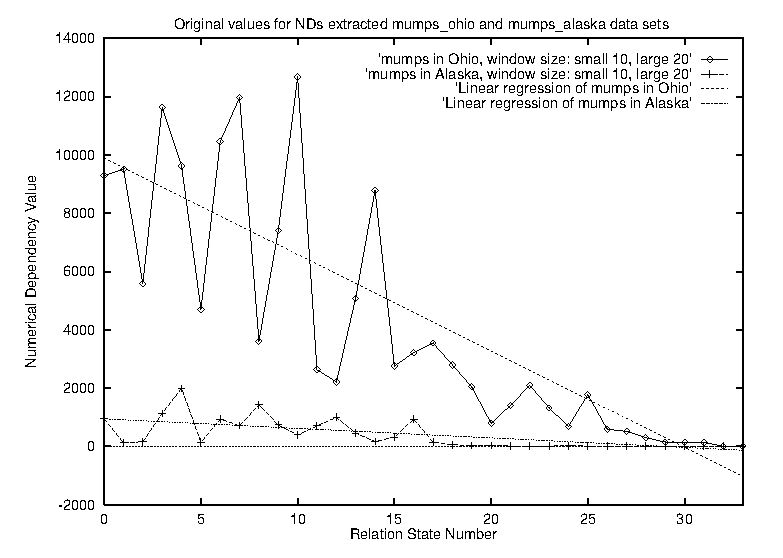
\includegraphics{figures/mumps_postv.eps}}}
\caption{\label{graph:mumps_ohio_1}{Original data values of mumps
cases in Ohio and Alaska from 1957 - 1989}}
\end{figure}

The results obtained for a small sequence size of 5 years and a large
size of 10 years were $\Delta_{mp} \models$ \resp{10}{5} ($ohio\downarrow_r \wedge^0 alaska\downarrow_r$)
together with persistence results of the following abbreviated form
\pers{10}{5} ($ohio\downarrow_r \wedge^0
alaska\downarrow_r$). Clearly, these results tell us 
that the number of cases in mumps is falling, continuously, without
significant fluctuation.  
Applying a simple pattern matching algorithm for comparing exact
trend within a sequence we find that \safe{12}
($ohio$ $\downarrow$ $\leadsto$ $ohio$ $\uparrow$ $\leadsto$ $ohio$ $\downarrow$) holds for Ohio. Therefore
although we have found the general trends to be downward there are
peaks within larger sequences.
For a comparison between the
number of cases in Alaska and Ohio we increased the sequence sizes to
12 and 20 and found, continuously throughout the sequence that the
following persistence rule holds: \pers{20}{12}
($ohio\downarrow_r \wedge^2 alaska\downarrow_r$). We see that the lag in
the downward trends (ohio lags alaska by 2 years) may provide an
indication that the number of 
cases falling is correlated with geographical regions. Obviously
expert knowledge is required to confirm this; \cite{fay98b} discusses
issues of correlation versus causality noting that it is generally not
clear in which situations correlation can lead to causality. It may be
foolish to infer a causal relationship solely on the basis of the
discovery of a lagged correlation. This is the subject of much study
with further references provided in \cite{gmp97}.

\smallskip
A complete description of the series is provided by ($ohio\downarrow_r
\wedge^1 alaska\downarrow_r$) $\leadsto$ ($ohio\downarrow_r
\wedge^2 alaska\downarrow_r$). We find the same rule from applying
discordance instead of linear regression. This rule concisely presents
the behaviour of the sequence. It is obtained from three 12 year sequences
with some overlap (there is 33 years of data) and compressed, for
clarity, so that $\sigma \leadsto \sigma$
becomes $\sigma$. We  
omit presentation of such description rules for longer time series.
We can see from these simple results how properties of NDs over time
can be succinctly characterised within our logic. We now move on to a
slightly more interesting example.

\medskip



\begin{figure}
\centerline{\scalebox{0.7}{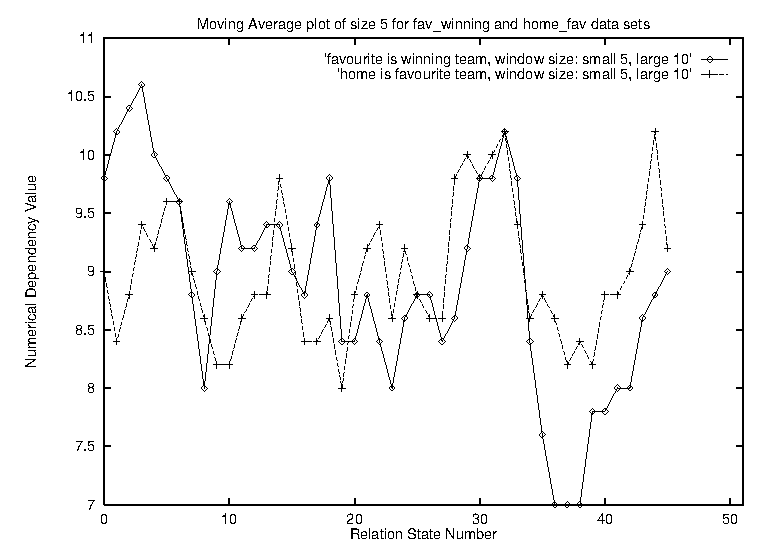
\includegraphics{figures/fav_winning_postv.eps}}}
\caption{\label{graph:profb_1}{Moving Average data set values of two NDs
from NFL season data 1989-1991}}
\end{figure}



In Figure~\ref{graph:profb_1} we present the changing ND values for
two NDs obtained from relations containing Football Data. Each week of
the season, for three seasons from 1989 to 1991, details of team
results were stored in a database together with details of the
favourite team for each match. We obtained two NDs from the relation
$YEAR$  $WEEK$ $\to^k$ $FAV\_TEAM\_WIN$ and $YEAR$  $WEEK$ $\to^k$
$HOME\_FAV$. These NDs correspond to the number of favoured teams
winning and the number of home favourites, respectively, within a
particular week.
We note that each relation contained $YEAR$  $WEEK$
 $DAY$ representing the day the match was played
on. Figure~\ref{graph:profb_1} shows
the two lines relating to changes in each ND. We can see no clear
trend in this figure for moving averaged data.

\medskip

For the two NDs we found the following property from the moving
average record of points with each moving average of size 5,
$\Delta_{NFL} \models$ \pers{10}{5} ($HOME\_FAV$ $\uparrow_r \wedge^0$
$FAV\_TEAM\_WIN$ $\uparrow_r$) suggesting that an
increase in the home team winning is correlated with an increase in
the favourite team winning. This persistence property expresses the fact
concisely and we can perhaps infer from this that the home teams are
most often the favourite team. Additionally, we examined the original
and differenced data set for patterns in sequences of 5 weeks and
found none. It is 
clear that the nature of the data contains no underlying trend 
expressing only the strong correlation between NDs.

\medskip

Before presenting the results obtained from time series data we
formally define the moving blocks bootstrap.

\subsection{The Moving Blocks Bootstrap}\label{subsec:tr_mbb}
\index{Moving Blocks Bootstrap}
\index{Bootstrap Resampling}


We introduce the Moving Blocks Bootstrap for verification of short
range event rules and provide details of its efficacy discussing the
results we found from its application in later sections.

\begin{definition}[Moving Blocks Bootstrap for Relation Sequences]\label{def:mbb}
\begin{rm}
Given a relation sequence $\{ r_1, r_2, \ldots, r_N \}$
we construct blocks of relations where $MB_t$ is a block containing
$b$ relations such that $MB_t = \{ r_t, r_{t+1}, \ldots, r_{t+b-1} \}$
and there are $N - b+ 1$ blocks where $t = 1, 2, \ldots, N-b+1$. We
then resample $k$ moving blocks uniformly with replacement from $\{
MB_1, MB_2, \ldots, MB_{N-b+1} \}$ where $N \sim bk$. This may be repeated any number of times.$\quad\Box$
\end{rm}
\end{definition}

\smallskip

\begin{figure}[ht]
\centerline{\scalebox{0.7}{\includegraphics{../Event_theory/mbb.eps}}}
\caption{\label{fig:mbb} All possible blocks of size 4 for a relation sequence}
\end{figure}

The moving blocks bootstrap forms an empirical distribution and this
distribution is the proposed bootstrap approximation. For a block
length $b$ all possible contiguous blocks of length $b$ within the
time series are available for selection. In \cite{et93} each moving
blocks bootstrap sample has an AR(1) model fitted to it to estimate
the parameter $\beta$. Results decreased upon an increase in the block
size, perhaps allowing us to infer that dependency was based on the
previous few points only (to any significant degree). The potential to
sample all possible contiguous blocks of a given size $b$ allows all
possible relationships of length less than or equal to $b$ to be sampled.


\subsection{The Moving Blocks Bootstrap for Large Data Sets}\label{subsec:tr_vlmbb}
\index{Moving Blocks Bootstrap}
\index{Bootstrap Resampling}


We now propose a new Moving Blocks Bootstrap for creating resamples
when either the temporal relation sequence or the time series contain
too many points for a resample to obtain meaningful results. For
example this may be a stock over 10 years. We may form a series of
values, which are fixed in ordering, so that this 10 year sequence may
be compressed into resamples of, say, 2 years each. This will then create a
manageable sequence size for property discovery across multiple
resampled sequences.

\begin{definition}[Moving Blocks Bootstrap for Large Relation Sequences]\label{def:vlmbb}
\begin{rm}
Given a relation sequence $\{ r_1, r_2, \ldots, r_N \}$ we construct a
resampled relation sequence of size $n$, where $N \gg n$, with the
order of the resampled relation sequence preserved from the original
data set.
We construct blocks of relations where $MB_t$ is a block containing
$b$ relations such that $MB_t = \{ r_t, r_{t+1}, \ldots, r_{t+b-1} \}$
and there are $N - b+ 1$ blocks where $t = 1, 2, \ldots, N-b+1$. 
We then divide the sequence into $R$ regions where $R = \frac{N}{n}$.
From each region $R_i$, $0 \le i \le R-1$ we resample 1 moving block
uniformly from $\{ MB_{(i*n)+1}, MB_{(i*n)+2}, \ldots,
MB_{(i*n)+n-b+1} \}$ and append 
the block to our resampled sequence. Order is therefore preserved for
$n$, a given 
size. This may be repeated any number of times. $\quad\Box$
\end{rm}
\end{definition}

\smallskip

\begin{figure}[ht]
\centerline{\scalebox{0.7}{\includegraphics{../Event_theory/vlmbb.eps}}}
\caption{\label{fig:vlmbb}A large relation sequence and a resample}
\end{figure}

Given that the random block selection for the moving blocks bootstrap
for large relations is order preserving we must be careful in our
random block selection to ensure that we do not initially select a
block at the end of the sequence to which no blocks can be
appended. To remedy this we propose that the sequence is divided into
a number of regions $n$, from Definition~\ref{def:vlmbb}. From these
regions we select one block randomly. For example, a 10 year sequence
may be divided into 24 regions, of 5 months each, from which a block
of one month is selected from each. This would then allow reasonable
knowledge discovery on a manageable sequence with relationships
between either NDs or time series preserved within blocks and the
 ordering of the sequence is preserved in the
resamples. Alternatively, we could use standard moving blocks
resampling with smaller sample sizes and sorting each resample into
the correct temporal order; this would create more randomness in the
resamples. 

\section{Time Series Data Results}\label{sec:tr_tsares}
\index{Time Series Data Results|(}


We now examine more complex temporal data sets. We 
assume that the data is restricted to numerical data alone, although
if the data were stored in a suitable manner then NDs
could easily apply. When analysing time series we are not seeking to
discover what a complex statistical analysis could not; indeed much of
our logic is based on statistical functions. Instead we are looking
for a concise representation that might convey specific properties
which hold at a certain time or throughout time and we express these
with our logic. The logic details properties in a machine
understandable form. 


\medskip

For the following study we focused on financial stocks from the FTSE
100. We analysed stocks in similar sectors seeing if there are general
properties from which we can infer information, concentrating on
financial, oil and retail sectors. We highlight some of the results
found and remark that all applications discovered possibly useful
properties. In the following we initially present results based on each category
of data, discussing the results with respect to the sequence size
selected; we follow this with a discussion of how these properties
might relate to the data they represent in the real world. A summary
of results is presented for each data set in
Tables~\ref{tab:tr_arg_deb_res}, ~\ref{tab:tr_bp_sh_res},
and~\ref{tab:tr_al_hfx_res}. As a precursor to this discussion we
remark that the absence of a property with respect to sequence sizes
chosen by the user, when evaluated with results for other sequence
sizes, may itself tell us much about the data set.

\section{Case Study I}\label{sec:tr_case1}

We present results for Debenhams ($db$) and the Arcadia Group ($ag$),
summarised in Table~\ref{tab:tr_arg_deb_res}, in an extended form
which highlight characterisation of the discovery of
property. Subsequent studies are abbreviated to avoid repetition and
we refer to this sequence as $\Delta_{ad}$. Due to the similarity
between regression and discordance results, we concentrate on results
obtained using linear regression. We note that we are now dealing
exclusively with time series and not ND values; this is primarily due
to the availability of time series data and, as we have seen, the
limited availability of data satisfying ND sets. We note that all
results are equivalent to those that may be found for ND sets in a
temporal relation sequence and could feasibly be expressed with NDs,
though this may often be impractical. 


{\line
\begin{table}[ht]
\begin{center}
\begin{tabular}{|c||c|} \hline 
\multicolumn{2}{|c|}{\bf Debenhams and Arcadia Group } \\ \hline
 Description of data set & 199 days of closing prices   \\ \hline
\multicolumn{2}{|c|}{In all formulae: Arcadia Group ($ag$) and
Debenhams ($db$)} \\ \hline
\multicolumn{2}{|c|}{\bf Trend Discovery} \\ \hline
Original Data Set       &  $\Delta_{ad}$ $\models$ \resp{80}{1} ( $ ag \downarrow$) \\
 			 & $\Delta_{ad}$ $\models$ \resp{80}{1} ($ db \uparrow$) \\\hline
\multicolumn{2}{|c|}{\bf Property Discovery} \\ \hline
Original Data Set	&   $\Delta_{ad}$ $\models$ $\bm^{160}$
 ( $ag \downarrow_r$ $ \wedge^{0}$ $db \downarrow_r$ ) $\leadsto$  ( $ag
 \downarrow_r$ $ \wedge^{0}$$ db \downarrow_r$)\\
			&  $\Delta_{ad}$ $\models$  \pers{10}{5}  ($ag
 \uparrow_r \wedge^{0} db \uparrow_r$ ) \\
			&   $\Delta_{ad}$ $\models$ \pers{20}{10}  ($ag \uparrow_r
 \wedge^{0} db \uparrow_r$ )\\
			&  $\Delta_{ad}$ $\models$ \pers{20}{10}  ($ag \downarrow_r \wedge^{0} db\downarrow_r$ )  \\
			&   $\Delta_{ad}$ $\models$ \pers{30}{15}
 ($ag \downarrow_r \wedge^{0} db \downarrow_r$ ) \\
			&  $\Delta_{ad}$ $\models$ \pers{40}{20}  ($ag
 \downarrow_r \wedge^{0} db \downarrow_r$)\\
			&  $\Delta_{ad}$ $\models$\pers{80}{40}  ($ag
 \downarrow_r \wedge^{0} db \downarrow_r$)\\
			&  $\Delta_{ad}$ $\models$ \resp{160}{80}  ($ag \downarrow_r
 \wedge^{0}\downarrow_r$)\\
			&  $\Delta_{ad}$ $\models$ \resp{160}{80}
 ($ag \uparrow_r \wedge^{1} db \downarrow_r$ )   \\ \hline
Moving Average          &  \\
Window size:3	&  $\Delta_{ad}$ $\models^3$ \pers{20}{10}  ($ag
 \downarrow_r \wedge^{0} db \downarrow_r$),
 found 12 times \\
Window size:8	&  $\Delta_{ad}$ $\models^8$  \pers{80}{40}  ($ag \downarrow_r
 \wedge^{0} db \downarrow_r$)     \\\hline
Moving Block Bootstrap          &  \\ 
Block Size: 5	&  $\Delta_{ad}$ $\models^3$ \pers{20}{10}  ($ag
 \downarrow_r \wedge^{0} db \downarrow_r$ )     \\
Block Size: 10	&  $\Delta_{ad}$ $\models^{3}$  \resp{40}{20}  ($ag
 \downarrow_r \wedge^{0} db \downarrow_r$)     \\
	&  $\Delta_{ad}$ $\models^{3}$   \resp{80}{20}  ($ag \downarrow_r
 \wedge^{0}\downarrow_r$) \\
All for MA Block Size:3		&  $\Delta_{ad}$ $\models^{3}$ \resp{80}{20}
 ($ag \uparrow_r \wedge^{0} db \uparrow_r$)    \\ \hline
Differenced Series        & \\
		  & $\Delta_{ad}$ $\models$  \resp{80}{20}  ($ag
 \downarrow_r \wedge^{0} db \downarrow_r$) \\ 
		&   $\Delta_{ad}$ $\models$  \resp{80}{20}  ($ag
 \uparrow_r \wedge^{0} db \uparrow_r$)  \\ \hline
2nd Order Differenced Series      & \\
		    &  $\Delta_{ad}$ $\models$  \resp{80}{20}  ($ag
 \uparrow_r \wedge^{0} db \downarrow_r$)\\ 
		&   $\Delta_{ad}$ $\models$ \resp{80}{20}  ($ag
 \downarrow_r \wedge^{0} db \uparrow_r$)    \\ \hline
\end{tabular}
\end{center}
\caption{\label{tab:tr_arg_deb_res} Results for 199 days of Arcadia and
Debenhams Group }
\end{table}
}

\subsection{Original Data Analysis}\label{subsec:tr_analysis}

Properties extracted from the original data set are based solely on
the original data values upon which our property discovery algorithms
are applied. We first discuss looking for trends as properties. We see
in Table~\ref{tab:tr_arg_deb_res} that we obtained safety trends, for
a sequence 
size 80, \resp{80}{1} ($ag \downarrow$) for the Arcadia Group and \resp{80}{1}
($db$ $\uparrow$) for Debenhams. This states that in every 80 day sequence
there is at least one day when the stock goes up or down! This may seem
obvious but these two results together suggest that Debenhams might be
performing better than Arcadia. The procedure to obtain these naive trend
rules uses a simple pattern matching algorithm. We also found 
persistence rules of the form 
 \pers{20}{10}  ($ag \uparrow_r \wedge^{0} db \uparrow_r$ ) and  \pers{20}{10}
($ag \downarrow_r \wedge^{0} db \downarrow_r$ ). The former
persistence rule was 
discovered at five points in the complete sequence and the latter was found to
hold at the very beginning of the series. This corresponds with the
actual values which are generally within a downward trend apart from
an initial upward trend depicted by their moving averages in Figure~\ref{graph:deb_199_2}. Increasing the sequence size shows that
persistence rules for upward trends do not hold at all for larger
sequence sizes and so we conclude that upward trends within the series
are short and that the general trend is down, exemplified by
\pers{80}{40} ($ag \downarrow_r \wedge^0 db \downarrow_r$). Similarly,
the safety 
trend descriptions indicate that Debenhams might be performing better
that Arcadia.
			

\subsection{Moving Average Analysis}\label{subsec:tr_mav_analysis}
\index{Moving Averages}
\index{Jackknife Resampling}

The goal of creating a moving average of a time series is to smooth
the series so that outliers, potentially caused by noise or outside
effects, have a weakened influence on the data discovery
process. They are widely used in stock data analysis \cite{rm97}.
 We conducted experiments with a jackknife procedure for moving
average smoothing, 
whereby the moving averages for each sequence are calculated
successively with one data point removed and then averaged. We obtained a
slight increase in smoothing over the standard moving average but not
enough to justify the additional computational cost in its use and so
this was not employed. 

\smallskip

Moving average results in general back up the results provided by the
original data set. We note that smoothing tends to obscure short
term trends so that persistence or guarantee rules which hold in the
original data set may not hold for a moving average
series. Additionally, the size of the window for moving 
averages increases the {\em spreading} effect of a single data
point. To illustrate we found far fewer properties for larger moving
average windows. Figure~\ref{graph:ma3_12} shows how a larger window
size increases the spread for the moving averages, reducing the
amplitude of both peaks and troughs.


\begin{figure}
\centerline{\scalebox{0.7}{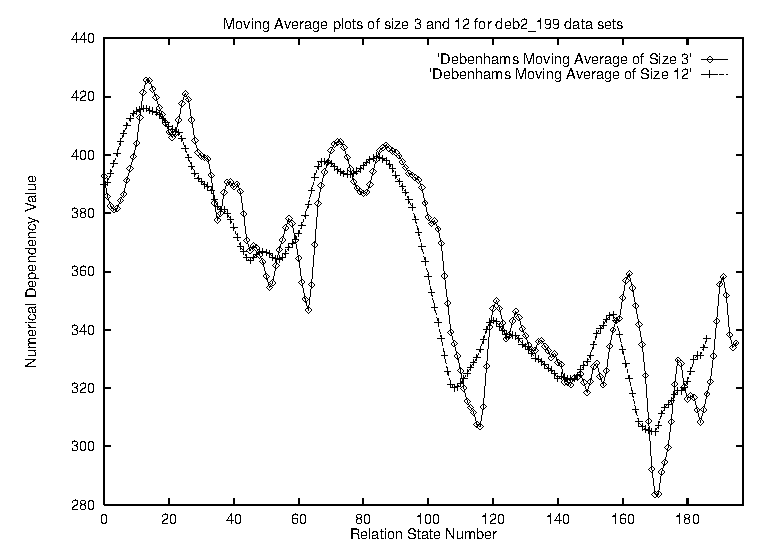
\includegraphics{figures/arg2_199_w20_b40_postv.eps}}}
\caption{\label{graph:ma3_12}{Moving Average Data
values for two window sizes, 3 and 12}}
\end{figure}


\subsection{Differenced List Analysis}\label{subsec:tr__diff_analysis}
\index{Differenced List}

In Time Series Analysis differencing is used by statisticians to
remove trend from a series, as we outlined in Section~\ref{sec:tl_tsa}.
Similarly we may obtain the differenced values for a data set upon
which we run our property detection algorithms. This may lead to the
discovery of properties which then represent seasonal and not trend
behaviour. We refer to Table~\ref{tab:tr_arg_deb_res} which
present some results for differenced lists. Due to the complex nature
of stock behaviour we can not be sure if the properties for
differenced lists detail seasonal or just noisy behaviour. The result
of a first differencing provides very similar results to the original
and moving average properties. Namely, that the behaviour of the two
stocks is closely related with response and persistence properties
detecting either joint upward or downward trends. Extending this to a
second order differencing we find that this shared behaviour is no
longer discovered. What can we infer from this?  For a conclusive
answer we would have to ask a fund manager, however, we note
that perhaps their seasonal behaviour is not related or that the
stocks are affected by different events outside of their
relationship. In such a way we can use our algorithms for the
discovery of seasonal properties.


\subsection{Moving Blocks Bootstrap Analysis}\label{subsec:tr_mbb_analysis}
\index{Moving Blocks Bootstrap}

The moving blocks bootstrap, defined in Section~\ref{subsec:tr_mbb},
is used within time series analysis for model creation based on the
assumption that temporal relationships do not occur for a time longer
than the size of the blocks used to create the moving blocks
resamples. The moving blocks resamples may then be recreated many
times to obtain a model based on these resamples. We created moving
blocks resamples of our time series. Interesting properties were found
and though we believe some properties for some resamples to be
spurious we could have removed these via repeated application of the
moving blocks bootstrap and intersection of the results.
Applying the moving blocks bootstrap also allows for properties to be
discovered which may be violated in sequences without such a
rearrangement, perhaps caused by noise.

\medskip

The order of the moving blocks resamples is random. It is therefore
highly likely that spurious trends may be found for the moving blocks.
\resp{80}{20} ($ag \downarrow \wedge^{0} db \downarrow$ ) and
\linebreak \resp{80}{20}
($ag \uparrow \wedge^{0} db \uparrow$ ) were both found with a block size
of 10 days. This implies, we believe, two things. Firstly, that the
behaviour of the two stocks is closely related both sharing either
upward or downward trends. Secondly, the difference between small and
large sequence sizes is quite significant implying that it is likely
that blocks will occur to create an upward trend shown in the second
response rule. The data miner needs to choose sequence sizes carefully
in such cases. For a block size 5 we found \pers{20}{10} ($ ag \downarrow$
$\wedge^0$ $ db \downarrow$ ), which backs up both the original and moving
average results. The variation of block size allows us to make
conclusions about the nature of the trends. For 5 and 10 days we found
properties with upward or downward trends suggesting that these stocks
possess trend behaviour longer, in general, than these block
sizes. This is, however, a feature of the financial market in general.


\section{Case Study II}\label{sec:tr_case2}

We present results for two oil stocks BP (bp) and Shell Oil (sh),
summarised in Table~\ref{tab:tr_bp_sh_res}, in an abbreviated form.

{\line
\begin{table}[ht]
\begin{center}
\begin{tabular}{|c||c|} \hline 
\multicolumn{2}{|c|}{\bf BP and Shell } \\ \hline
 Description of data set & 242 days of closing prices   \\ \hline
\multicolumn{2}{|c|}{In all formulae: British Petroleum ($bp$) and Shell ($sh$)} \\ \hline
\multicolumn{2}{|c|}{\bf Trend Discovery} \\ \hline
\multicolumn{2}{|l|}{\bf Techniques} \\ \hline
BP   & $\Delta_{oil}$ $\models^w$ $\bm^{15}$ \diam$^1$ ($bp
\downarrow$) \\
	& $\Delta_{oil}$ $\models$ $\bm^{50}$ \diam$^4$
($bp \downarrow$  $\leadsto$  $bp \uparrow$ $\leadsto$ $bp \downarrow$
$\leadsto$ $bp \uparrow$ ) \\
Shell & $\Delta_{oil}$ $\models$ $\bm^{15}$ \diam$^1$ ($sh\uparrow$) \\
	& $\Delta_{oil}$ $\models$ $\bm^{50}$ \diam$^3$ ($sh\uparrow$
$\leadsto$ $sh\downarrow$ $\leadsto$ $sh\uparrow$ )  \\\hline
\multicolumn{2}{|c|}{\bf Property Discovery} \\ \hline
Original Data Set  & $\Delta_{oil}$ $\models$ \pers{30}{15}  ($bp \downarrow_r
		\wedge^{0}sh\downarrow_r$), found 7 times \\
		&  $\Delta_{oil}$ $\models$ \resp{45}{15}  ($bp\downarrow_r \wedge^{0}sh\downarrow_r$)\\
		&  $\Delta_{oil}$ $\models$ \pers{60}{30}  ($bp\downarrow_r \wedge^{0}sh\downarrow_r$)\\ 
		&  $\Delta_{oil}$ $\models$ \resp{90}{45}  ($bp\uparrow_r \wedge^{0}sh\uparrow_r$) \\
		&  $\Delta_{oil}$ $\models$ \resp{180}{90}
		($bp\uparrow_r \wedge^{0}sh\downarrow_r$) \\ 
		& $\Delta_{oil}$ $\models$ \resp{180}{90}  ($bp\uparrow_r \wedge^{0} sh\uparrow_r$) \\ \hline
Moving Average  & $\Delta_{oil}$ $\models^3$ $\bm^{180}$
 ( $bp\downarrow$ $ \wedge^{0}$ $sh\downarrow$ ) $\leadsto$  ( $bp\downarrow_r$ $ \wedge^{0}$$sh\downarrow_r$) \\
Block Size: 3 	&  $\Delta_{oil}$ $\models^3$ \pers{60}{30}  ($bp\uparrow_r \wedge^{0}sh\uparrow_r$)\\
		&  $\Delta_{oil}$ $\models^3$ \pers{60}{30}  ($bp\downarrow_r \wedge^{0}sh\downarrow_r$) \\
Block Size: 8 	&  $\Delta_{oil}$ $\models^8$ \pers{30}{15}  ($bp\downarrow_r \wedge^{0}sh\downarrow_r$),
		found 7 times\\
Block Size: 10	&  $\Delta_{oil}$ $\models^{10}$ \pers{60}{30}  ($bp\uparrow_r \wedge^{1}sh\uparrow_r$) \\\hline
Moving Block Bootstrap          &  \\
Block Size: 15		&  $\Delta_{oil}$ $\models^{8}$ \resp{60}{30}  ($bp\downarrow_r \wedge^{0}sh\downarrow_r$) \\ 
Block Size: 25		&  $\Delta_{oil}$ $\models^{8}$ \resp{100}{50}
		($bp\downarrow_r \wedge^{0}sh\downarrow_r$) \\
All for MA Block Size: 8 & \\ \hline
Differenced	&  $\Delta_{oil}$ $\models$ \resp{60}{30}  ($bp\downarrow_r \wedge^{0}sh\downarrow_r$)
		\\  \hline
2nd Order Differenced	&  $\Delta_{oil}$ $\models$ \resp{60}{30}  ($bp\downarrow_r
		\wedge^{0}sh\uparrow_r$) \\ 
		&  $\Delta_{oil}$ $\models$ \resp{60}{30}  ($bp\uparrow_r
		\wedge^{0}sh\downarrow_r$) \\ 
 			& $\Delta_{oil}$ $\models$  \resp{60}{30}  ($bp\downarrow_r
		\wedge^{0}sh\downarrow_r$) \\  \hline
\end{tabular}
\end{center}
\caption{\label{tab:tr_bp_sh_res}Results for 242 days of BP and Shell
		from Dec 1997 to Oct 1998} 
\end{table}
}

The original values again emphasise a strong relationship between the
two data sets at smaller sequence sizes. We experimented with large
sequence sizes and found 
\linebreak \resp{180}{90} ($bp \uparrow_r \wedge^0 sh \downarrow_r$).
Two points
about this are worth noting. Firstly, the disparity in trend in not
immediately clear from a graph, cf. Figure~\ref{graph:bp_11mn_1},
which exhibits much similarity. The initial upward trend of BP stocks
may be viewed as {\em masked} by a number of short term downward
trends which the properties suggest.
Secondly, the data set consists of
only 242 points (days). Yet we are looking for sequences of 180 days
which implies that there is no sequence which does not overlap with
another. This response rule is therefore perhaps not quite so strong
though still interesting. 

\medskip

Finally, we briefly refer to Table~\ref{tab:tr_al_hfx_res}. This
consists of stock prices for two newly converted building societies in
their first 100 days on the market. Though we found properties they do
not present themselves as showing much similarity. We can infer that
the behaviour of the market at the time of launch is itself more
important that what the company is. Tests showed that different stocks
over different time periods tend towards not discovering properties as
opposed to discovering properties which represent disparate
behaviour.  Additionally, of the properties discovered we see a number
of spurious lags which do not suggest strong related behaviour. This
is a validation of our discovery process. 
 
{\line
\begin{table}[ht]
\begin{center}
\begin{tabular}{|c||c|} \hline 
\multicolumn{2}{|c|}{\bf Halifax and A \& L Banks } \\ \hline
 Description of data set & 100 days of closing prices   \\ \hline
\multicolumn{2}{|c|}{In all formulae: Alliance \& Leicester ($al$) and
Halifax ($hfx$)} \\ \hline 
\multicolumn{2}{|c|}{\bf Trend Discovery} \\ \hline
 A \& L   & $\Delta_{ha}$ $\models$ $\bm^{10}$ \diam$^1$ ($al$ $\uparrow$) \\
 Halifax  & $\Delta_{ha}$ $\models$ $\bm^{10}$ \diam$^1$ ($hfx$ $\downarrow$)\\
	&  $\Delta_{ha}$ $\bm^{20}$ \diam$^1$ ($hfx$ $\uparrow$) \\
		&        \\\hline
\multicolumn{2}{|c|}{\bf Property Discovery} \\ \hline
Original Data Set  & $\Delta_{ha}$ $\models$  \resp{60}{30}  ($al\downarrow_r \wedge^{6}hfx\downarrow_r$)\\
		& $\Delta_{ha}$ $\models$  \resp{60}{30}  ($al\uparrow_r \wedge^{-3}hfx\downarrow_r$)\\
		\hline
Moving Average  & $\Delta_{ha}$ $\models^5$  \pers{20}{10}  ($al\uparrow_r \wedge^{0}hfx\uparrow_r$)\\
Block size: 5	& $\Delta_{ha}$ $\models^5$  \resp{60}{30}  ($al\uparrow_r \wedge^{-3}hfx\downarrow_r$) \\
		& $\Delta_{ha}$ $\models^5$  $ \bm^{60}$ ( $al\downarrow_r$ $ \wedge^{6}$
		$hfx \downarrow_r$)\\ \hline
Moving Block Bootstrap          &  \\ 
Block size: 5	& $\Delta_{ha}$ $\models^5$  \pers{20}{10}
		($al\downarrow_r \wedge^{0}hfx\uparrow_r$)\\ 
MA Block size:5 & \\ \hline
\end{tabular}
\end{center}
\caption{\label{tab:tr_al_hfx_res} Results for first 100 days trading
		of Halifax and Alliance \& Leicester Banks }
\end{table}
}

\subsection{Real-World Analysis}\label{sec:tr_real_analysis}


\begin{figure}
\centerline{\scalebox{0.7}{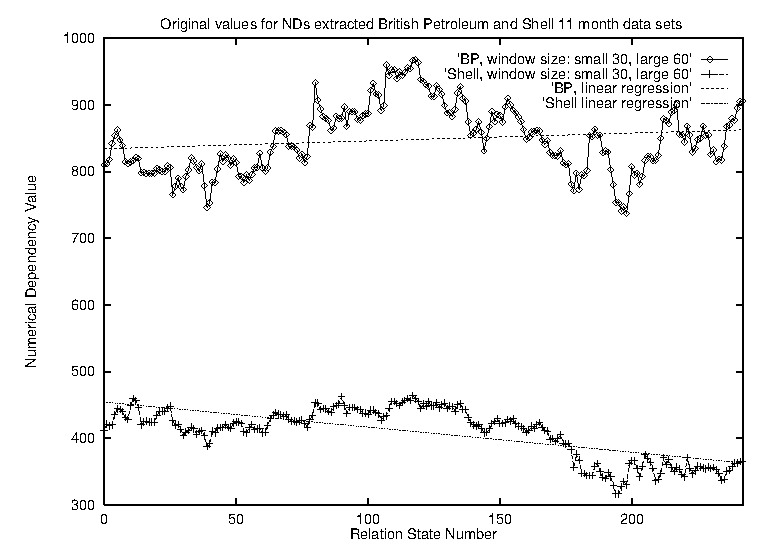
\includegraphics{figures/bp_11mn_sh_11mn_postv.eps}}}
\caption{\label{graph:bp_11mn_1}{Time series of BP and
Shell from 1 Dec. 1997 to 1 Nov. 1998}}
\end{figure}

Our first analysis
focuses on BP and Shell. Under a story entitled ``bad times for the
oil industry'' in the Lex column of the Financial Times, November 4
1998, it was discussed how the oil industry has suffered in recent
months though some recent results (third quarter) posted by BP show
that a 35\% drop in profits is good news in comparison with a more
than 50\% drop by Shell prices. We can see from
Figure~\ref{graph:bp_11mn_1} that BP ($bp$) has been outperforming
Shell ($sh$) in
terms of recent performance. We discovered however that the stocks are
related in short term performance, as we would expect. We found that
in Jan and Feb the following persistence property held \linebreak \pers{90}{60}
($bp$ $\uparrow_r \wedge^0$ $sh$ $\uparrow_r$), a period of gradual
rise in both stocks. We also found that \linebreak \pers{60}{30} ($bp$
$\downarrow_r \wedge^0$ $sh$ $\downarrow_r$) holds from day 160 in
Figure~\ref{graph:bp_11mn_1}, relating to the downward trend that
begins in May. With a smaller
sequence similar results 
were obtained though we also discovered that \pers{10}{5} ($bp$ $\downarrow_r
\wedge^0$ $sh$ $\uparrow_r$) held in September 1998; this opposite behaviour
may be due to external influences.

\medskip

In Figure~\ref{graph:deb_199_2} we show the moving averaged sequence
for two companies, Debenhams ($db$) and the Arcadia Group ($ag$) since
January 28 1998. On January 28 1998 Debenhams demerged from its former
owner the
Arcadia Group. We can see from Figure~\ref{graph:deb_199_2} that
recently Debenhams has performed better 
than Arcadia due to, based on expert opinion, the fact that Debenhams
sells many different goods whereas Arcadia concentrates more on fashion and
is expected to perform poorly in the light of a recession. In August
1998, corresponding with a downturn in the economy, we found
\pers{30}{15}  ($db$ $\downarrow_r \wedge^0$ $ag$ $\downarrow_r$) and
for the recent good performance of Debenhams we found \pers{10}{5} ($db$
$\uparrow_r \wedge^0$ $ag$ $\downarrow_r$), amongst other rules. The
regression coefficient used to determine trend may be significantly
small. However the trend still exists and we can subscript trends by
their regression value or even extend this to a {\em fuzzy} value to denote the
significance of the trend.   


\begin{figure}
\centerline{\scalebox{0.7}{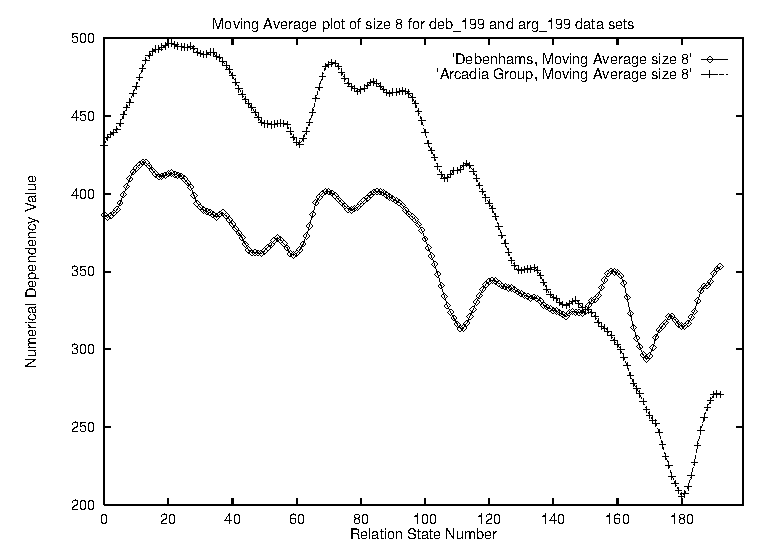
\includegraphics{figures/deb_199_w15_b30_postv.eps}}}
\caption{\label{graph:deb_199_2}{Moving Average values for
Debenhams and Arcadia Group since demerger on Jan 28 1998}}
\end{figure}


It is imperative that the two sequence sizes are well chosen by the
user. It would help if the user had expert knowledge of any kind of
seasonality duration. If $n > \frac{m}{2}$ where $n$ is the
smaller sequence size and $m$ the larger then there will be an overlap
of at least one point in all $n$ size subsequences of $m$. This is to
be avoided and is advisable as a lower bound on the sequence size
relationship. 

\smallskip

 For BP and Shell we found no properties for sequence
sizes of less than 15 days on a moving blocks resampled sequence. This
may imply that trends relate to longer term behaviour.
We
found within all results that we tested the moving blocks results
confirmed previously found persistence results and occasionally
presented spurious response properties. Repeated application to
numerous moving block sequences and intersecting the results removed
these spurious properties. Similarly differencing provided similar
results in the data we tested; this may be due to forcing sequences
and studying local linearity removes the need for longer term trend
removal.
\index{Time Series Data Results|)}


\section{Moving Blocks Bootstrap for Large Relations}\label{sec:mbb_large}



\begin{figure}
\begin{minipage}{7cm}
\centerline{\scalebox{0.5}{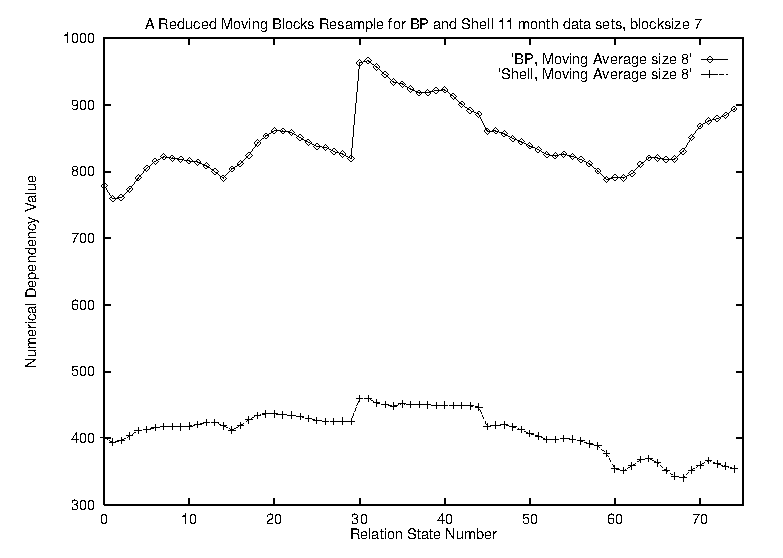
\includegraphics{figures/bp_11mn_w30_b60data_postv.eps}}}
\caption{\label{graph:bp_11mnfixblock1}{Reduced moving blocks
samples for BP and Shell moving average data, 78 points from 11
regions and blocksize of 7 points}}
\end{minipage}
\hfill
\begin{minipage}{7cm}
\centerline{\scalebox{0.5}{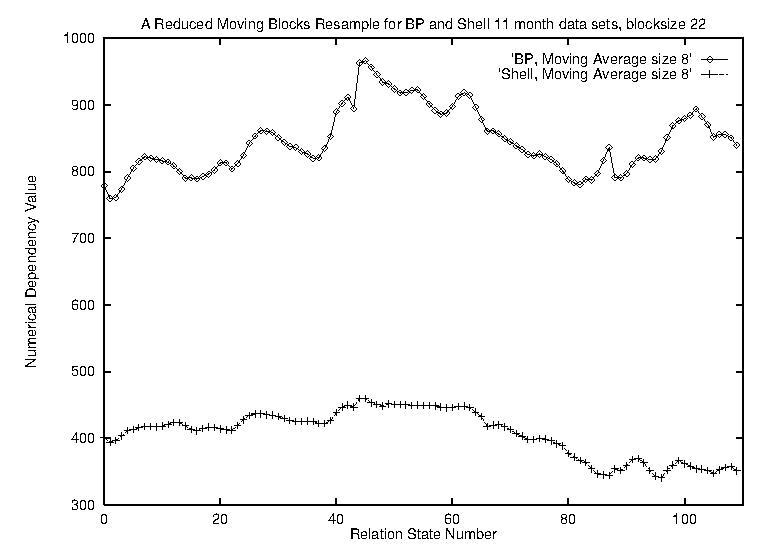
\includegraphics{figures/bp_11mn_w45_b90data_postv.eps}}}
\caption{\label{graph:bp_11mnfixblock2}{Reduced moving blocks
samples for BP and Shell moving average data, 110 points from 5
regions and blocksize of 22 points}}
\end{minipage}
\end{figure}


The use of the moving blocks bootstrap for large relations allows
smaller resampled relation sequences to be created from the original data set. 
We can see in Figure~\ref{graph:bp_11mnfixblock1}, for example,
a moving block resample of only 78 points from the original data set
of 242 points, which closely resembles the original data set. The need
for repeated iterations of the moving blocks samples is shown in the
results found. We found $\Delta_{oil} \models$ (\pers{30}{15}
($bp \uparrow_r \wedge^0  sh \uparrow_r$)), and, in abbreviated form, \resp{30}{15} ($bp \uparrow \wedge^0
sh \uparrow$), \resp{30}{15} ($bp \downarrow \wedge^0
sh \downarrow$), and \resp{30}{15} ($bp \uparrow \wedge^0
sh \downarrow$) in one resample, which was not found in the original data
set. We also found \resp{90}{45} ($bp \uparrow \wedge^0
sh \uparrow$) and \resp{90}{45} ($bp \downarrow \wedge^0
sh \downarrow$), the latter of which was not found for the original
data set.

\medskip

We draw the following conclusions from using the moving blocks
bootstrap for very large relations:
\begin{itemize}
\item A visual analysis shows that Figures~\ref{graph:bp_11mnfixblock1} and
~\ref{graph:bp_11mnfixblock2} in comparison with
Figure~\ref{graph:bp_11mn_1} of the original data set show the
similarities for the two smaller resampled sequences. Such similarity can be 
exploited for knowledge discovery when a series contains a significant
number of points to obtain a valuable {\em synopsis} of the sequence.
\item That the resampled original, and possibly even the resampled
moving average, data sets of reduced size, contains too many fluctuations, and as such allows the
generation of properties which may be {\em generally} false of the
data. For example, two resampled blocks may be concatenated and they
may violate, or satisfy, a trend which holds, or does not.
\item The use of the moving blocks bootstrap to cut down the number of
points needed to examine for the discovery of properties, is, like the
property discovery process itself, highly dependent on the choice of
both {\em block size} and the {\em region size} from which the blocks
are selected. If the block size is too small with respect to the
region size it will not reflect trends sufficiently well. It it is too
large then it will closely resemble the original sequence, which we
might as well use in this situation. There is of course the additional
problem of selecting a suitable blocksize in relation to the sequence
sizes for property discovery. A blocksize smaller than a sequence size
is more likely to result in fewer properties discovered, particularly
when the resampled series is much smaller than the original.
\item Even for a small number of points the reduced moving blocks
bootstrap is able to detect relationships, and properties, across
series reasonably well.
\end{itemize}

Resampling to create reduced size sequences is valuable when the data
set is too large to mine in full for property satisfaction.

\section{Critical Analysis}\label{sec:tr_crit_an}

Our methodology for the discovery of properties has a number of
problems. Particular properties are more likely to be discovered for
particular sequence size choices. A response rule \resp{m}{n} is much
more likely to hold when $m \gg n$ wherein the guarantee property
\diam$^n$ is given more time in which to occur. Clearly, the data
miner has the choice of setting these parameters.

\medskip

Another questionable area is that whether all properties discovered
are interesting. This is certainly not true. For example, we must be
very careful with guarantee properties to ensure that they are not
presented as knowledge discovery without good reason. This begs the
question, what makes a property interesting? As properties become more
complex they are more likely to represent an interesting feature of
the dataset. We must be careful with properties that are not {\em
boxed}, i.e., not safety properties. For example, an {\em ordered
persistence property} of the form $\sigma_1 \leadsto$ \pers{m}{n} $\sigma_2$
can be found for any persistence property apart from the very start of
the time sequence, given that $\sigma_1$ can be an arbitrary formula
which is true in some sequence before \pers{m}{n} $\sigma_2$ holds.
Therefore it is of little value in knowledge
discovery terms. However, if this property occurs similarly at regular
points(within $\bm^{p}$) then we have discovered something potentially
very interesting about the data.

\medskip

The use of time series statistics has been shown to be both efficient and
useful. We have found our representation of lags in the logic to be
equivalent, though developed independently by what we considered to be a requirement, to the representation in time series of {\em lag
operators} \cite{end95}, where the value is ignored and only the lag
itself is important. We conducted some tests to examine the efficacy
of the lag. This was particularly important as most properties
discovered found 0 lag. We overlapped our time series by a number of
points $n$ and then removed the extraneous $n$ points at the beginning
and end of the respective series. We found similar properties to hold
but with the lag to be the same value as the overlap. For example, we
found \pers{30}{15} ($ag \downarrow \wedge^{0} db \downarrow$ ) became
\pers{30}{15} ($ag \downarrow \wedge^{3} db \downarrow$ ) when the overlap
was 3 points for the retail data set. As we extended
this the number of properties discovered decreased due to the lower
likelihood of behaviour reoccurring at regular intervals. Additionally,
for small sequences, overlaps also resulted in fewer properties. Upon
the advice of \cite{ko90} we restricted lags to $\frac{n}{4}$ given
that otherwise stronger lags are found at the highest lag length where
there are far fewer points to correlate.  \cite{end95} suggests
beginning with the longest plausible lag length over which there may
be a possible relationship. 


\begin{figure}
\centerline{\scalebox{0.7}{\includegraphics{figures/timeplot_200_postv.eps}}}
\caption{\label{graph:prop_disc_time}{Time for discovery of
response and persistence properties for varying small and large
sequence sizes and small varying only (for a large sequence size)
within a 398 point data set}}
\end{figure}

In Figure~\ref{graph:prop_disc_time} we provide details of the times
required for discovery of response, \resp{m}{n}, and persistence, \pers{m}{n},
properties for different sequence 
sizes. We found that sequence size increasing for both $m$ and $n$ at
a fixed rate (with $m = 2n$) was
similar to increasing only the sequence size $n$ with respect to
property discovery for large sequence size $m = 200$. This is due to
most of the computation 
time working on the discovery of safety and guarantee properties with
respect to $n$. Also there are small fluctuations in the time
required. We found this was due to some sequences satisfying fewer
initial safety and guarantee properties leading to faster checking
time for response and persistence
properties. Figure~\ref{graph:prop_disc_time} shows that properties
can be discovered very efficiently.

\medskip
In Section~\ref{subsec:temp_mine} we discussed a number of alternative
approaches to temporal data mining. We now compare our approach to
that of \cite{bt98} which uses a restricted temporal logic in conjunction with
probabilities and an interestingness measure for rule discovery from
input strings. In the example we 
now discuss \cite{bt98} obtain the probability of an event $e$ from
dividing its frequency in a string by the total length of the string
such that each {single} event has an interestingness of exactly 1.
Within the domain of a {\ttb sendmail\tte} program, having 31
commands, rules were discovered, such as ({\em sigblock} ${\cal N}$
{\em setpgrp}) ${\cal N}$ {\em vtrace} 
with an attached interestingness value of 43.16, where
{\em sigblock}, {\em setpgrp}, and {\em vtrace} are commands within the
program. Additionally ({\em sigblock} ${\cal B}_k$ {\em stepgrp}) ${\cal B}_k$
{\em vtrace} is also discovered with the same interestingness value
suggesting that $\cal N$ would be redundant if the subscript $k$ were
given explicitly. Our logic may, if applied to a similar domain,
represent the latter rule as ({\em sigblock} $\leadsto$ {\em setpgrp})
$\leadsto$ {\em vtrace}, assuming 
that we allow program commands as atoms. We can also
use properties to denote how often these rules occur within a
given period of time. For example, a response rule within every two
minute period is expressed by \resp{120}{n} ({\em sigblock} $\leadsto$
{\em setpgrp}) $\leadsto$ 
{\em vtrace}, where $n$ is the time to execute these commands. An extension
to our work could be the creation of our own {\em interestingness}
measure based on a property being more interesting if the ratio of the
smaller to larger sequence size is closer to 1. This could also be
applied from the larger sequence size to complete sequence size.
\cite{bt98}
also restrict the size of maximum string length for discovery such
that the rules found cover only a small size of the original input
string. Rules within sequences allow for discovery over longer time
periods as we have seen; this is aided by our use of regression.

\section{Similarity Assessment}\label{sec:tr_sim_ass}
\index{Time Series Similarity}

Much recent work looking at assessing the similarity of two time
series \cite{alss95,frm94,dgm97,rm97}, as discussed in
Chapter~\ref{chap:review}, concentrates on transformations applied to
Fourier sequence representation of a time series.  As a novel
contribution to this field we add our use of property discovery for
similarity assessment. From suitable sequence sizes we
discover properties which may represent related behaviour across
sequences telling us about trends, lags, and seasonal events.

\medskip

\cite{rm97} apply Euclidean distance
to moving average time series to see if two time series are similar. 
\cite{dgm97} applies transformation functions so that the scaling of
the two time series being compared need not necessarily be the same
over the same number of points. This is a useful feature which would
also be of value for property discovery. Time series are considered
similar if there exists an approximate transformation function which maps one
series to the other. \cite{dgm97} considers linear functions only. We
now propose another definition of similarity based on sequence sizes
such that two sequences are similar if all properties discovered for a
particular sequence size depict equivalent behaviour. For example,
both moving average trends or seasonal behaviour after differencing
would always be equivalent for both time series within all properties
found. The work of \cite{alss95} does not allow outliers and requires
sequences to be of the same length whereas
property discovery from moving averages would have the effect of
already weakening any outliers. Our form of knowledge discovery will
also have the advantage in that properties may be discovered which
correspond to a particular range of the sequence within which they may
exhibit similar behaviour before diverging.
Most studies of similarity
would not provide a decent result in this instance, particular if we
are looking for a linear transformation function.  Though we do not
explicitly allows translation across time points of our time series
this, as we have shown, is represented by the presentation of lags or
lead values within series. 

\medskip

Finally, we remark that if a querying system were implemented for our
logic the similarity would be able to be enumerated via a set of
queries which may or may not hold.

\section{Discussion}\label{sec:tr_disc}



If a database query language were to incorporate the ability to search
for properties within a temporal database then any DB user would be
able to ask questions concerning possible properties that he suspects
might hold in the data. We have shown that this can be achieved using
our logic in polynomial time. The current range of statistical
functions available in DBMS need only minimal extension to include time
series functions and then it would be entirely feasible to express
relationships in a readily understandable form such as that of our
logic.
 
\medskip
 
We have presented our logic for NDs in temporal sequences. Results
applied to temporal relation sequences and time series have shown our
logic capable of providing succinct characterisation of the data to a
{\em system user}. The response and persistence properties that we
discovered are both useful and 
valid and may be applicable in a decision support
environment. Properties discovered within a DBMS might be
desired to hold for all future points in which case they could be
elevated to the status of integrity constraints. 
Extensions to this work include the implementation of a
querying system and additional algorithms for property discovery.

\medskip
We presented a generic algorithm for the discovery of knowledge using
the temporal classification of properties and then refined this to a
specialised algorithm for response and persistence rule discovery. The
algorithm is generic in that it applies to all discovery which uses
the classification hierarchy, of which our model in
Figure~\ref{fig:model2} is one particular instance.
The similarities between
these and the generic algorithms given in \cite{man96,man97} point to
similarities within the data mining model. Work on a unified theory of
data mining will require a set of generic mining algorithms which can
be specialised for many different approaches \cite{jmw96}.
\medskip 

The goals of \cite{bt98} were to generate unexpected predicates,
expressed in a restricted temporal logic, from sequential databases or
strings. This has application in rule discovery from categorical data
whilst our logic relies on numerical data alone, though in the case of
NDs this may be based on categorical data. The restriction of a
maximum string length is similar to our requirement of a given
sequence size. A sequence of size $n$ satisfying $\sigma_1 \leadsto
\sigma_2$ differs only from $\sigma_1 {\cal B}_k 
\sigma_2$ found in a string of size $n$ in that we allow overlap,
assuming that $\sigma_1,\sigma_2$ occur in sequences. The need
for restriction is 
that the interestingness measure is always higher for longer sequences
implying that a rule representing the complete input string is always
the most interesting whereas our motivation is to enable property
discovery, possibly relating to, say, seasonal behaviour.
Both properties and measures, such as interestingness, are of value
within data mining.

\smallskip

Much recent knowledge discovery research has been concerned with
finding out if two time series are in some sense similar
\cite{frm94,alss95,dgm97}. Our logic has the expressive power to represent
similarities as properties or standard sentences of the logic from
which we can easily deduce similarities between two time series. As an
avenue for further work it
would be interesting to expand this using, perhaps, intersections of
properties found for similarity assessment.
